%THIS SECTION FOCUSES ON THE IDEAS BEHIND THE SCHEME (MORE ABOUT CONCEPTUAL DESIGN)

\section{Privacy-Aware LBA}
As discussed above, with a tremendous growth of smartphone usage, LBA has become a very promising market. However, privacy concerns, especially location privacy concern, in a certain extend, discourage a portion of users to participate in this market. We argue that if LBA service doesn't compromise users location privacy, it will be much more broadly accepted and its market will be further extended. The key idea behind our privacy-aware LBA model is to keep location information locally on user's smartphone instead of disclosing it to LBAS as in traditional model. The mobile devices perform some simple computation to figure out which ads should be served in current spatial context and then $privately$ requests those ads from LBAS. Later on, ads reports, which tells how many times a certain ads is displayed, are collected in such a way that leaks no sensitive information. By guaranteeing privacy in each phase of the LBA serving process, we can protect users' location privacy. In this section, we propose \codename, a framework for location-privacy aware LBA and discuss its underlying concepts. 

\subsection{Architecture}
\codename proposes two changes to the traditional LBA architecture. The first component of \codename is a small service called $mPrAd$ running in user's smartphone. Unlike traditional model of LBA where ads-sponsored mobile applications establish connections and retrieve ads directly from LBAS, in our model, they just need to call $mPrAd$ service.
Specifically, when an ads-sponsored application is in use, it is bound to $mPrAd$ to retrieve ads. $mPrAd$ first collects exact location information from sensor (i.e. GPS sensor) and perform the \textit{space encoding} (subsection \ref{subsec:space_encoding}) to get a location index. It then establishes a secure channel to SC and submits the request via that secure channel. The SC receives the request, performs a \textit{private ads retrieval} (detailed in \textit{Algorithm 1}). The SC then returns the ads to $mPrad$'s. Upon receiving response from SC, $mPrAd$ forwards a set of ads to mobile applications. For every ads displayed, the application sends an acknowledgement to $mPrAd$. Based on the acknowledgement, $mPrAd$ can keep track of how many times each ads is displayed. At the end of a billing period, $mPrAd$ builds billing vectors and reports them anonymously to the LBAS(subsection \ref{subsec:billing}). We sequentially discuss details of these procedures in the following subsections. 

$mPrAd$ contains two secret key, one for performing space encoding and the other to encrypt billing vector. The reason to delegate these tasks to a small independent service like $mPrAd$ is that ads-sponsored applications are not always trusted. There are incentives for such applications to leak user's sensitive information, which is user's location in this context. Mobile applications can be designed to look benevolent to pass vetting procedure of apps publisher but become malicious once it is installed on user's phone \cite{jekyll}. Hence, ads-sponsored application should not be granted access to location sensor, which is required in the first place for space-encoding process, unless there is an explicit need of location information to facilitate its authorized activities. The other reason is that there are so many apps developers that distributing a set of secret keys required in our model incurs many complications. By introducing $mPrAd$, we can avoid such secret key distribution problem. One more reason is that there may be several ads-funded application running in the same smartphone; and running a single $mPrAd$ to serve all of those ads can save computational and communication cost compared to each application perform ads retrieval separately. 


The second change involves the presence of a trusted Secure Processor SC (figure \ref{fig:architecture}). Specifically, SC is required to be installed on LBAS and every request to LBAS is routed through this SC. Note that this SC is able to read and write data to LBAS's database.


% a figure is very good way to demmostrate
\begin{figure*}[placement specifier]
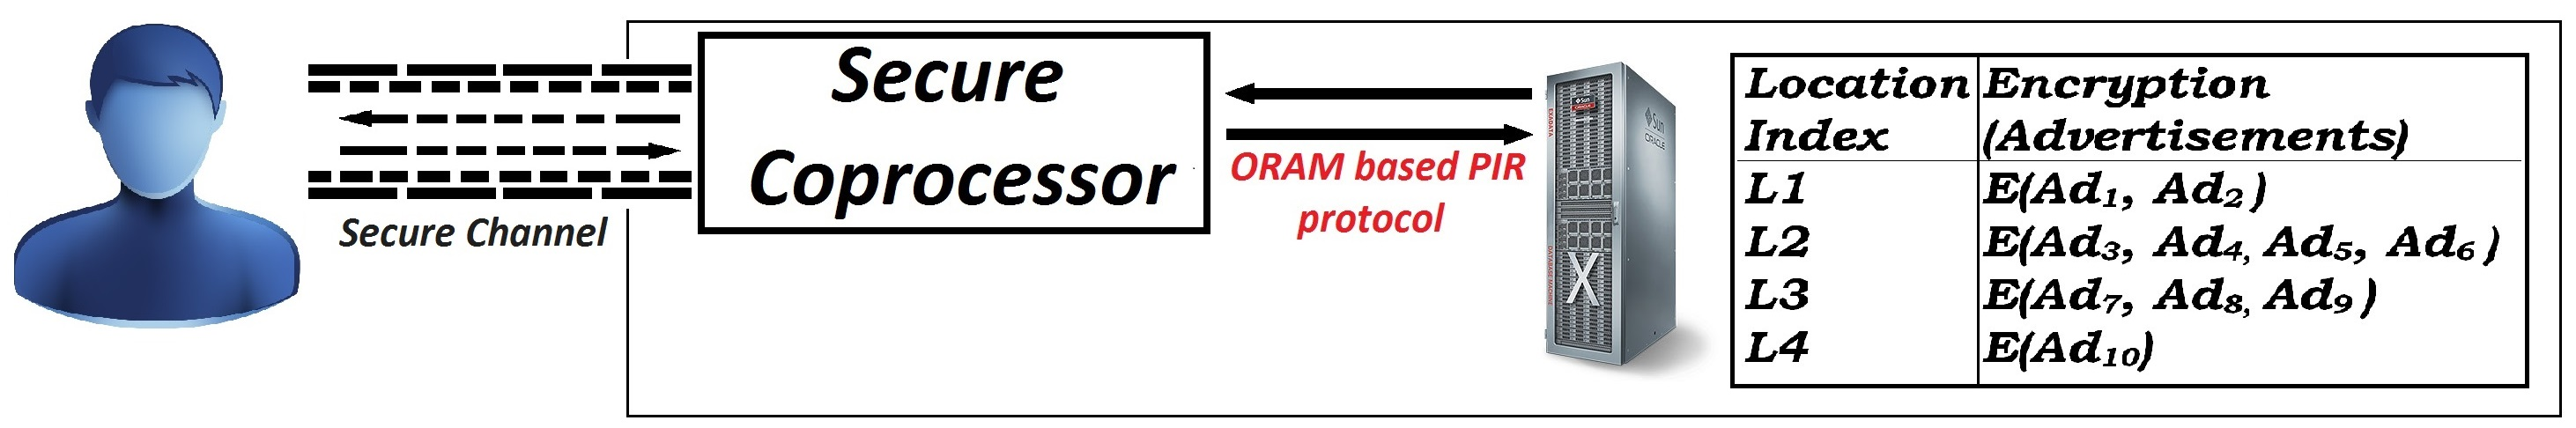
\includegraphics[scale=0.22]{figures/architecture_img.jpg}
\caption{Private ads retrieval}
\label{fig:architecture}
\end{figure*}





\subsection{Space Encoding} 
\label{subsec:space_encoding}
Unlike traditional LBS model in which the users send their location information to the server and let the server decide on which services they will be served, the client device in our model makes such a selection on its own. We consider the traditional mode of LBA as \textit{Server assigning ads} while we classify our approach as \textit{User selecting ads}. We assume that LBAS stores ads as a dictionary of form $\langle$\textit{Location Index - Set of Ads}$\rangle$ where \textit{Location Index (LI)}  is calculated using a one-way function based on the ads' locations. Specifically, assume that a user is at location $l$, instead of asking the LBAS "please send me ads near $l$", the client calculates the location index $li$ that represents $l$ and then retrieves from LBAS ads whose index is $li$. That is, we change the ads query to the ads selection. We refer to the process of calculating location index as \textit{space encoding}. 

The space encoding needs designing so that it is a one-way transformation. A transformation is one-way if forward computation could be performed easily while backward or invert computation is computationally impossible. Moreover, since this space encoding is performed on users' mobile devices, its computational cost in term of time and computational resources should be low. The reason for this constraint is that the ads selection process needs real-time performing and that smartphone has limited computational power compared to a server. Another observation is that the basic nature of ads selection is to select not only an ads located exactly as user's location, but also ads in her proximity. Moreover, each user has different preference on a range of the proximity; i.e. some users prefer to retrieve ads within a small area surrounding them while other users opt to retrieve ads in a slightly larger area. Thus, the space encoding must preserve the locality and clustering aspects of spatial data. In order to satisfy the above mentioned requirements, we adopt a Hilbert curve based space-encoding technique proposed in \cite{Space_Transformation} as a space encoder in our model. We briefly present the notion of \textit{space filling curve} and summarize the technique.

Space filling curves is the one that visits all points in space without crossing itself. This class of curves retains the proximity and locality aspects of the spatial data. Hibert curves \cite{hibert_curve} is one of the most famous member of this class due to its excellence in preserving distance and clustering characteristics of the spatial data. The space encoding technique introduced in \cite{Space_Transformation} uses a set of four parameters to form a \textit{Space Decryption Key SDK}. The four parameters comprise of the curve's starting point $(X_0, Y_0)$, curve orientation $O$, curve order $N$ and curve scale factor $F$. It is proven in the paper that this space encoder is secure, i.e. it is computationally impossible to invert the encryption without the knowledge of $SDK$. Given ads are indexed based on \textit{Location Index} calculated by this space encoding and all ads contents are encrypted properly, LBAS has no information to locate the user when it serves her request.


In the real-worlds, many ads are located in the same area. For example, there are many products from different brands offered in one supermarket, and many supermarkets co-located in the same neighborhood. \codename groups all ads that are in the same area into one set, and then indexes such a set with the location index of that area. (This reasons our assumption on LBAS storing ads database as a dictionary of form $\langle$\textit{Location Index - Set of Ads}$\rangle$). Note that the size of such an area is a sensitive parameter in our framework. We discuss the effect of this parameter in subsection \ref{subsec:square_size}.
Without loss of generality, let us presume that there is a minimum bounding rectangle that surrounds the entire region. Then, we divide such a rectangle into $x$ unit squares, each of which represents an area. Note that there will be areas (unit squares) containing ads and some others don't. \codename only keeps track of areas that contain ads. Besides all ads submitted by advertisers, \codename stores a special ads record which is to be served to users having no ads in their proximity.

Our space encoder utilizes space-filling curve, which reserves neighborhood and locality of spatial data object; i.e. if two spatial object are near each other, their spatial indices calculated by our space encoder will also very close to each other. Because of this very interesting property, our framework allows extra flexibility in serving ads. Specifically, users can decide on a range of the area in which they want to retrieve ads. $mPrAd$ treats a wide area as an union of several unit squares. In case a user opts to be served ads in an area comprising of many unit square, let us say $s$ for example, $mPrAd$ will send $s$ requests to LBAS. $mPrAd$ only needs to calculate one location index of the user's current location; other location indices of surrounded unit squares are inferred based on the calculated on. For example, if the user opts to retrieve ads in an area that is 3 times larger than default unit square, and her current location's index is $l$, then $mPrAd$ will sends 3 requests with indices \textit{l-1}, $l$, \textit{l+1} to LBAS.



\subsection{Private Ads Retrieval} 
\label{subsec:PIR}
So far, we have discussed how the idea of \textit{User selecting ads} can be practical using space-transformation technique. Given this technique alone, user's location privacy is protected in snapshots. Without the knowledge of how the space-encoding calculate the location index, LBAS cannot invert the transformation and infer actual location of the users. Thus, for a single request, user's location information is kept private. However, her privacy is still suffered from correlation attack in which the LBAS observes the access frequencies and history trajectories of the user. It can make quite good inference on her locations based on those observations and external geographic knowledge of the area. In order to further improve the privacy guarantee and completely prevent any potential sensitive information leakage, we propose to utilize PIR technique in Ads retrieval. Our target is to enable client app to retrieve ads without the LBAS knowing what ads it has served.

The key challenge in our model is to privately retrieve selected ads from the LBAS. We adopt Hardware-based PIR techniques to obtain the privacy in ads retrieval due to its optimal communication and computation costs compared to cryptographic PIR. It is worth mentioning that placing a trust on a secure coprocessor (SC) installed on LBAS is fundamentally different from trusting the LBAS. In case of the SC, we only need to trust its designer, while the trust that we place on LBAS involve credits paid to not only its designer but also its administrator and all other applications installed on it. Another observation is that SC is a tamper-resistance hardware device which is programmed to perform some specific operations. It is easier to vet the SC compared to screening the LBAS.

Several SC-based PIR protocols employ \textit{random permutation} techniques to first permute the original database DB into permuted one ($DB_p$) and later on access $DB_p$ to privately retrieve records \cite{PIR_SC_2006, PIR_SC_betterShuffling, PIR_SC_betterShuffling_2008}. Even though these approaches are able to obtain optimal communication and computation costs, they need to carry out an \textit{offline preprocessing} to reshuffle the entire database periodically. The cost of this offline reshuffling is not trivial and thus make these protocols inapplicable in our context. We introduce some modifications to the random permutation to avoid these overheads. As the result, our private ads retrieval is able to achieve optimal communication and almost optimal computation cost without periodically performing the reshuffling. 
The key insight is instead of performing one big reshuffle periodically, we slightly change the database after each retrieval. Such a change should be minimum to keep the processing cost low, yet still significant enough to nullify LBAS's correlation and access pattern attacks. We now present the SC-based Private Ads Retrieval protocol.

\paragraph{The architecture}
An ads database $DB$, which comprises of $n$ records, is hosted on LBAS. SC is connected to LBAS and able to read and write records from and to the LBAS's database. SC comprises of a private memory $M$ with a limited storage capacity. As SC is tamper-resistant, it follows that its private memory is also trusted and LBAS cannot have any access to or observation on the content of the memory. Every request to LBAS is configured to be routed through SC. The role of the SC is to serve as a proxy sitting between users and LBAS. 


\paragraph{Protocol}
In the \textit{LBAS initialization} or \textit{pre-deploy} phase, the SC encrypts $n-k$ records using a randomized encryption and write them to the permuted $DB_p$ while keeping $k$ remaining records in its memory (k is chosen according to SC's memory capacity and $n-k$ to be encrypted records are chosen randomly). Note that those $k$ ads are cached in SC's memory in plain-text form; while other $n-k$ ads are saved in $DB_p$ in their cipher-text form. Thus, one ads record will have two form, plain-ads if it is in SC's memory, or cipher-ads if it is in $DB_p$ and it can only be of one out of two form at a time (since it is stored either in $M$ or $DB_p$ but not both).
The randomized encryption generates different cipher-text each time the same plain-text is encrypted. If the encryption is not randomized, the access frequency of ads is partially leaked to the LBAS. In order to keep track of the permutation of $n$ records in the original database $DB$,
SC maintains the mapping table $MapT$ in its private memory $M$. Specifically, each item $MapT[li]$  is a pair of form $<a, x>$ where $li$ is the location index of the original ads record, $x$ is a position of the cipher-ads in $DB_p$ and $a$ is the boolean value signaling whether position $x$ has been accessed. If an ads is stored in $M$ (in plain-ads form), the corresponding $a$ and $x$ are set to $-1$ since its cipher-ads is not stored in $DB_p$. We refer to the set of plain-ads stored in $M$ as $PA$. There are three possible values that an item $MapT[li]$ can take:

\begin{itemize}
\item \textit{MapT[li] = (-1, -1)}: the ads is in plain-ads form and is kept in $M$
\item \textit{MapT[li] = ( 0, x)}: the ads is in cipher-ads form, kept in $DB_p$ at position $x$. Position $x$ has $NOT$ been accessed before. This cipher-ads is marked as $unaccessed$ cipher-ads.
\item \textit{MapT[li] = ( 1, x)}: the ads is in cipher-ads form, kept in $DB_p$ at position $x$. Position $x$ has $ALREADY$ been accessed before. This cipher-ads marked as $accessed$ cipher-ads.
\end{itemize}


In the \textit{online retrieval} phase, for each request, the SC will read from the $DB_p$ one \textit{unaccessed cipher-ads} and one \textit{accessed cipher-ads} to $M$. We refer to the set of \textit{unaccessed cipher-ads} as $uCA$ and a set of  \textit{accessed cipher-ads} as $aCA$.
Note that these cipher-ads are randomly chosen. It then randomly chooses two plain-ads from $M$, encrypts and write them to $DB_p$ to replace the two recently read cipher-ads in $DB_p$; i.e. they are written to the exact position of the recently read cipher-ads. These two positions are then marked as $accessed$. $MapT$ is updated accordingly after each retrieval. After all cipher-ads are marked as $accessed$, SC randomly leaves one as $accessed$ and remarks all remaining \textit{n-k-1} cipher-ads in $DB_p$ as $unaccessed$ to start a new round. 
Details of the online retrieval process are given in \textit{Algorithm} \ref{Alg:1} where random selection is denoted by $\xleftarrow{R}$ in \textit{Algorithm} \ref{Alg:1} while assignment is denoted by $\gets$ 

\begin{algorithm}
\label{Alg:1}
\vspace{-10pt}

\hrulefill
\vspace{-5pt}

 \textbf{Retrieve }(\textit{Location Index li})\\
 \vspace{-10pt}

\hrulefill

\If{li not in $Index\_List$}{
 $li$ $\gets$ $Default \ Index$\;
}

 \eIf{MapT[$li$] = (-1,-1)}{
 	U $\xleftarrow{R}$ uCA\;
 	A $\xleftarrow{R}$  aCA\;
 }{\eIf{MapT[$li$] = (0,x) }{
 	U $\gets$ $DB_p[x]$\;
 	A $\xleftarrow{R}$  aCA\;
 }{	
 	U $\xleftarrow{R}$  uCA\;
 	A $\gets$ $DB_p[x]$\;
 }
 }
  u $\gets$ Read(U)\;
  a $\gets$ Read(A)\;
  
  $result \gets$ PA[li]\;
  	 
  
  Write(u)\;
  Write(a)\;
  
  
  Update $MapT$ accordingly\;
  Return $result$ to the client\;	
 \vspace{-8pt} 
\hrulefill

\caption{Online Retrieval}
\end{algorithm}


\begin{algorithm}
\hrulefill
\vspace{-5pt}

 \textbf{Read }(\textit{cipher-ads c})\\
 \vspace{-10pt}
\hrulefill

 Read $c$ from $DB_p$ to $M$\;
 $pos \gets$ position of $c$ in $DB_p$\;
 $DB_p \gets DB_p - c$\;
 %Decrypt $C$ to get its corresponding plain-ads $P$ and save $P$ in $M$\;
 $p \gets$ Decrypt($c$)\;
 PA $\gets$ PA + $p$\;
 Return $pos$\;
 \vspace{-8pt} 
\hrulefill

\caption{Read}
\end{algorithm}




\begin{algorithm}
\hrulefill
\vspace{-5pt}

 \textbf{Write }(\textit{position x})\\
 \vspace{-10pt}
\hrulefill

 $p$  $\xleftarrow{R}$ PA\;
 $c \gets$ Encrypt($p$) \;
 $DB_p[x] \gets c$\;
 PA $\gets$ PA - $p$\;
\vspace{-8pt} 
\hrulefill

\caption{Write}
\end{algorithm}
 

Note that there are regions in which there is no advertisers publishing ads. To be able to deal with a situation in which users request ads from a non-ads area, SC keeps a list called $Index\_List$ which stores location indices of all ads records LBAS servers. Upon retrieving a request, it first checks if the requested location index is available. If it is not, SC will reassign the requested location index to a default value $Default\ Index$. Besides all ads published by Advertisers, LBAS keeps a special record whose index is \textit{Default Index} and content includes some particular advertisements that LBAS serves for free (for example, these advertisement could be from a charity organization or an advertisement of LBAS's own service).


\subsection{Billing and Accounting} 
\label{subsec:billing}

In order to bill the advertisers, LBAS must know how many times a certain ads is displayed (or clicked). Client apps need to report to LBAS which ads is clicked or displayed so that LBAS can charge advertisers and pay application developer accordingly. We refer to this feedback as \textit{ads-report}. However, we insist that it is necessary to hide the knowledge of what advertisements displayed on which users' mobile apps in other to guarantee users' location privacy. Thus, it is required that ads reports are collected in an anonymous way. Our intuition is that instead of each individual sending her ads report directly to LBAS and advertiser, a group of users first aggregate their ads report and only the aggregated information is sent to LBAS and advertiser. These pieces of accumulated ads reports won't reveal sensitive information of individual users but are sufficient to perform billing and accounting.

We take advantages of homomorphic encryption concept and \textit{k-anonymity} \cite{k-anonymity} to maintain the anonymity of ads reports. In detail, $mPrAd$ keeps counters of ads displayment of the form \textit{$<$Advertiser - Ads Counter$>$}. Within one billing period, whenever a counter for a specific advertiser reaches a predefined threshold \textit{maximum counter} $MC$, $mPrAd$ encrypts the counter using homomorphic encryption to get encrypted value $EC$, put it to a message of form \textit{$<$Advertiser-P-EC$>$} where \textit{P} is a number of peers the message has to be routed through before reaching LBAS and Advertiser and sends it to another peer. Initially, \textit{P} is set to 0. Upon receiving a message, the peer checks whether its own counter for that advertiser is greater than 0. If it is, it encrypts the value to get an encrypted value $EC_1$, resets the counter to 0, and then performs the summation of $EC$ and $EC_1$. It then updates $EC$ value in the message to the encrypted result of the summation, increases \textit{P} by one and check if \textit{P} now reaches a predefined threshold $MP$ (maximum peers). If \textit{P} is now equal to $MP$, it sends $EC$ to both LBAS and the corresponding advertiser. If \textit{P} is still smaller than $MP$, it sends the accumulated billing message to a next peer. In case the receiving peer's counter for the advertiser specified in the message is 0, it just increases \textit{P} by 1, and then based on the new value of \textit{P}, it will sends the billing message to LBAS and corresponding advertiser or to the next peer. At the end of billing period, client app encrypts and sends out every counters which are greater than 0 even if they haven't reached $MC$ yet. Since the time constraint in reporting billing information is quite flexible, these billing message transmitting could routed using Delay-Tolerant Network (DTN) \cite{DTN} to save energy and communication cost. Note that the selection of receiving peer is performed randomly using DTN technique, which increases the anonimity of the accumulated ads reports. In other to prevent one peer from inferring which ads are displayed on the previous peer, $mPrAd$ can pair each ads report which an empty ads report, i.e. ads report of an ads whose counter is 0.   Upon receiving billing counters of advertisers, LBAS, having secret key of the homomorphic encryption, decrypts them and update its billing database accordingly. Note that because billing information is also sent to advertisers so that they can verify the correctness of LBAS billing. 



%. Such aggregated information is a vector $v = (v_1, v_2,...,v_n)$ comprises of $n$ elements where $n$ is total number of ads that LBAS offers and $i^{th}$ element has a value equivalent to the number of times the $i^{th}$ ads is displayed (clicked). Then, \codename encrypts each component of $v$ using a homomorphic public key $pk$ to obtain a ciphertext vector $(E(pk, v_1), E(pk, v_2),...,E(pk, v_n))$ and sends this encrypted billing vector back to LBAS. Then, LBAS, given $pk$, can calculate the total amount of times ads are displayed. It then asks the SC, who has privatekey, to decrypt the aggregated billing vector. The SC is configured in such a way that it serves LBAS only one decryption per each month so that the LBAS cannot ask it to decrypt a billing vector of an indiviual since LBAS will loose the opportunity to decrypt aggregated billing vector. Note that secret key is kept secret from LBAS so that it cannot decrypt individual billing vector by itself.




\subsection{Security}
We claim that \codename can obtain strong location privacy. We justify this claim by sequentially proving that in delivering ads to users, \codename satisfies all three security metrics discussed in section \ref{sec:background}. In addition, the use of homomorphic encryption and k-anonymity concept in \codename 's billing procedure further fortifies our claim.

Given the presences of SC, there is no direct interaction between users and LBAS. The only interaction between LBAS and SC is facilitated through the private retrieval detailed in \textit{Algorithm 1}. That is, in the view of the LBAS, every request is exactly the same as each other no matter by whom it is issued. Thus, our technique satisfy the \textit{u-anonymity} metric.
Thanks to the space encoding as well as the randomized encryption and database permutation privately performed in each ads retrieval, LBAS cannot figure out which POI is actually received interest. That is, it doesn't know from where user sent their request. Thus, \textit{a-anonymity} is guaranteed. 
Finally, as described in \textit{Algorithm 1}, with respect to the view of LBAS, the SC performs exactly the same sequence of operations and (permuted) database access for every ads retrieval. Specifically, it reads one accessed record and one unaccessed record to its memory $M$, and then replace those two records with randomly chosen and encrypted item from $M$. Thus, we argue that our ads retrieval approach is \textit{data-oblivious}, which nullifies LBAS's ability of inferring any sensitive information based on database's access frequency. It is clear that our technique appreciates all three privacy metrics, \textit{a-anonymity}, \textit{u-anonymity}, and \textit{data-oblivious execution}.  In billing process, ads-reports are collected anonymously so that LBAS cannot learn which ads is displayed on which user's device. At this point, we claim that \codename leaks no sensitive information on users' actual location to untrusted party and hence, it achieves strong location privacy in providing LBA service.
